
\section{System Overview}

% ������LATEXдһƪ���ģ���Ҫ��˫����ʽ�м��������ͼ��:��\begin{figure}�м���*���ɣ�����\begin{figure*}  \end{figure*} ��

\begin{figure}[htb]
  \centering
 %\setlength{\abovecaptionskip}{-15pt}
 %\setlength{\belowcaptionskip}{-5pt}
    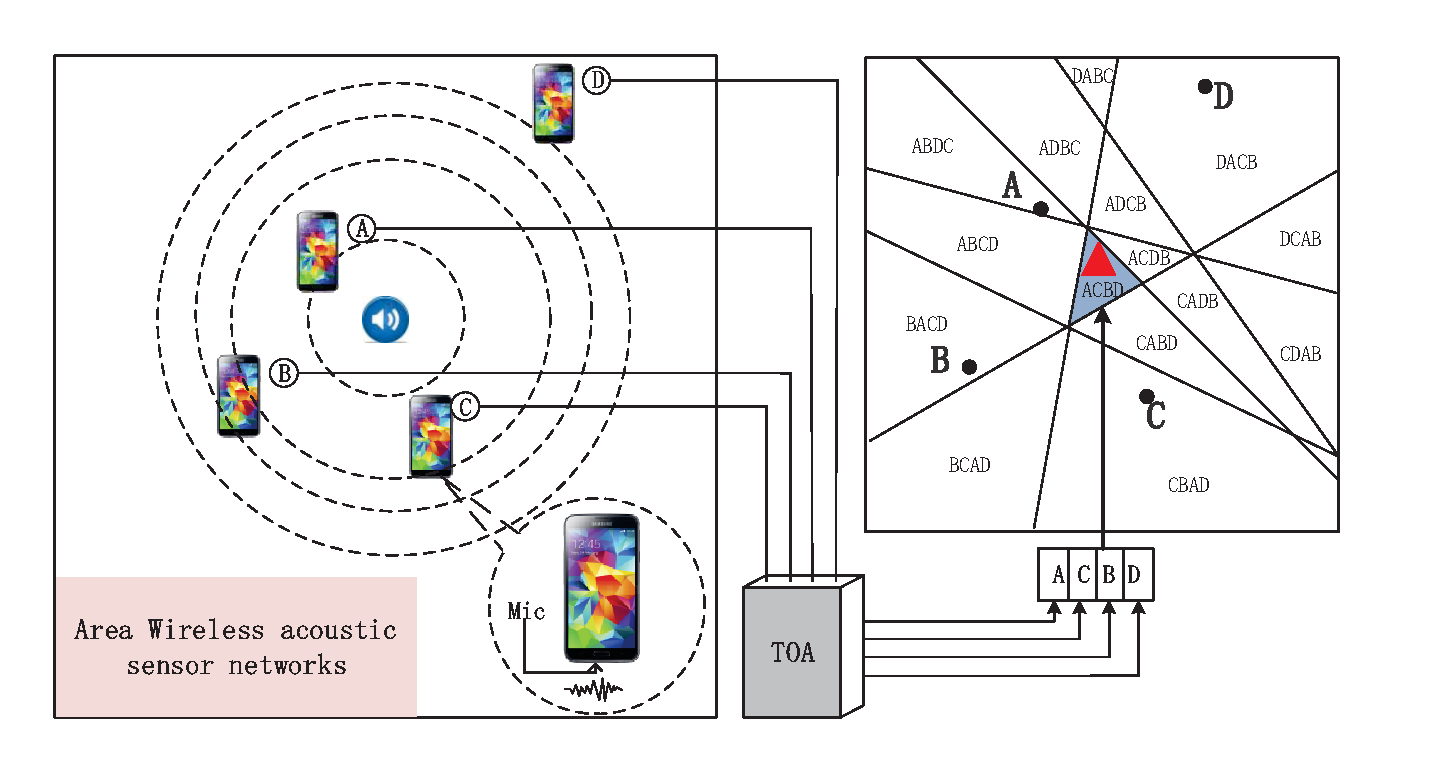
\includegraphics[height=4.5cm]{image/fig1.eps} 
    \caption{Overview of LPSBL}
 \label{overview}
    \end{figure}


In this section, we focus mainly on the system overview of our LPSBL system, which aims at locating an unknown node. 
Fig. 1 shows a layout of a sensor network with anchor nodes and the acoustic source.
We use circles to denote anchor nodes with known locations and the triangle to denote the acoustic source.
Assume that a 2D localization space consists of
$N$ reference nodes. Consider any two reference nodes and
draw a perpendicular bisector to the line joining their
locations. This perpendicular bisector divides the localization
space into two different regions that are distinguished
by their proximity to either reference nodes, as illustrated in
Fig. 1. Similarly, if perpendicular bisectors are drawn for
all pairs of reference nodes, they divide the localization
space into many regions.
All locations inside a region have the same location
sequence. If each region in the arrangement is represented by
its centroid, then there is a one-to-one mapping
between a location sequence and the centroid of the
region that it represents.

Briefly, sequence-based localization system works as follows. 
After the acoustic source generates a sound, anchor nodes detect the event sequentially at different time instances that naturally gives an ordering of related nodes, called a node sequence. 
For instance, in Fig. 1, when the acoustic source generates a wave, the node sequence $NodeSeq (A C B D)$ is obtained along the sound propagation. 
The location information of acoustic source is embedded within the node sequence. 
The node sequence of a given region is unique to that region.
By collecting all sensing results, locations of the acoustic source can be estimated by processing the node sequence. 

Specifically, as shown in Fig. 2, $NodeSeq (A C B D)$ can be obtained by time of arrival (TOA) information of the acoustic event.
Moreover, the TOA sequence ${t_A} < {t_C} < {t_B} < {t_D}$ is determined by the distance sequence ${d_A} < {d_C} < {d_B} < {d_D}$ from each node to the acoustic source $S$.

\noindent \textbf{Problem 1:} Assume that the location of acoustic source is known, the node sequence can be obtained by the distances from nodes to the acoustic source.

Sequence-based localization can be considered as an inverse problem of Problem 1, and described as:

\noindent \textbf{Problem 2:} Assume that the node sequence obtained from the measurement is known, estimate the location of an acoustic source.

    \begin{figure}[!htb]
    \centering
 \setlength{\abovecaptionskip}{-15pt}
                     \vspace{-5mm}  
 %\setlength{\belowcaptionskip}{-5pt}
    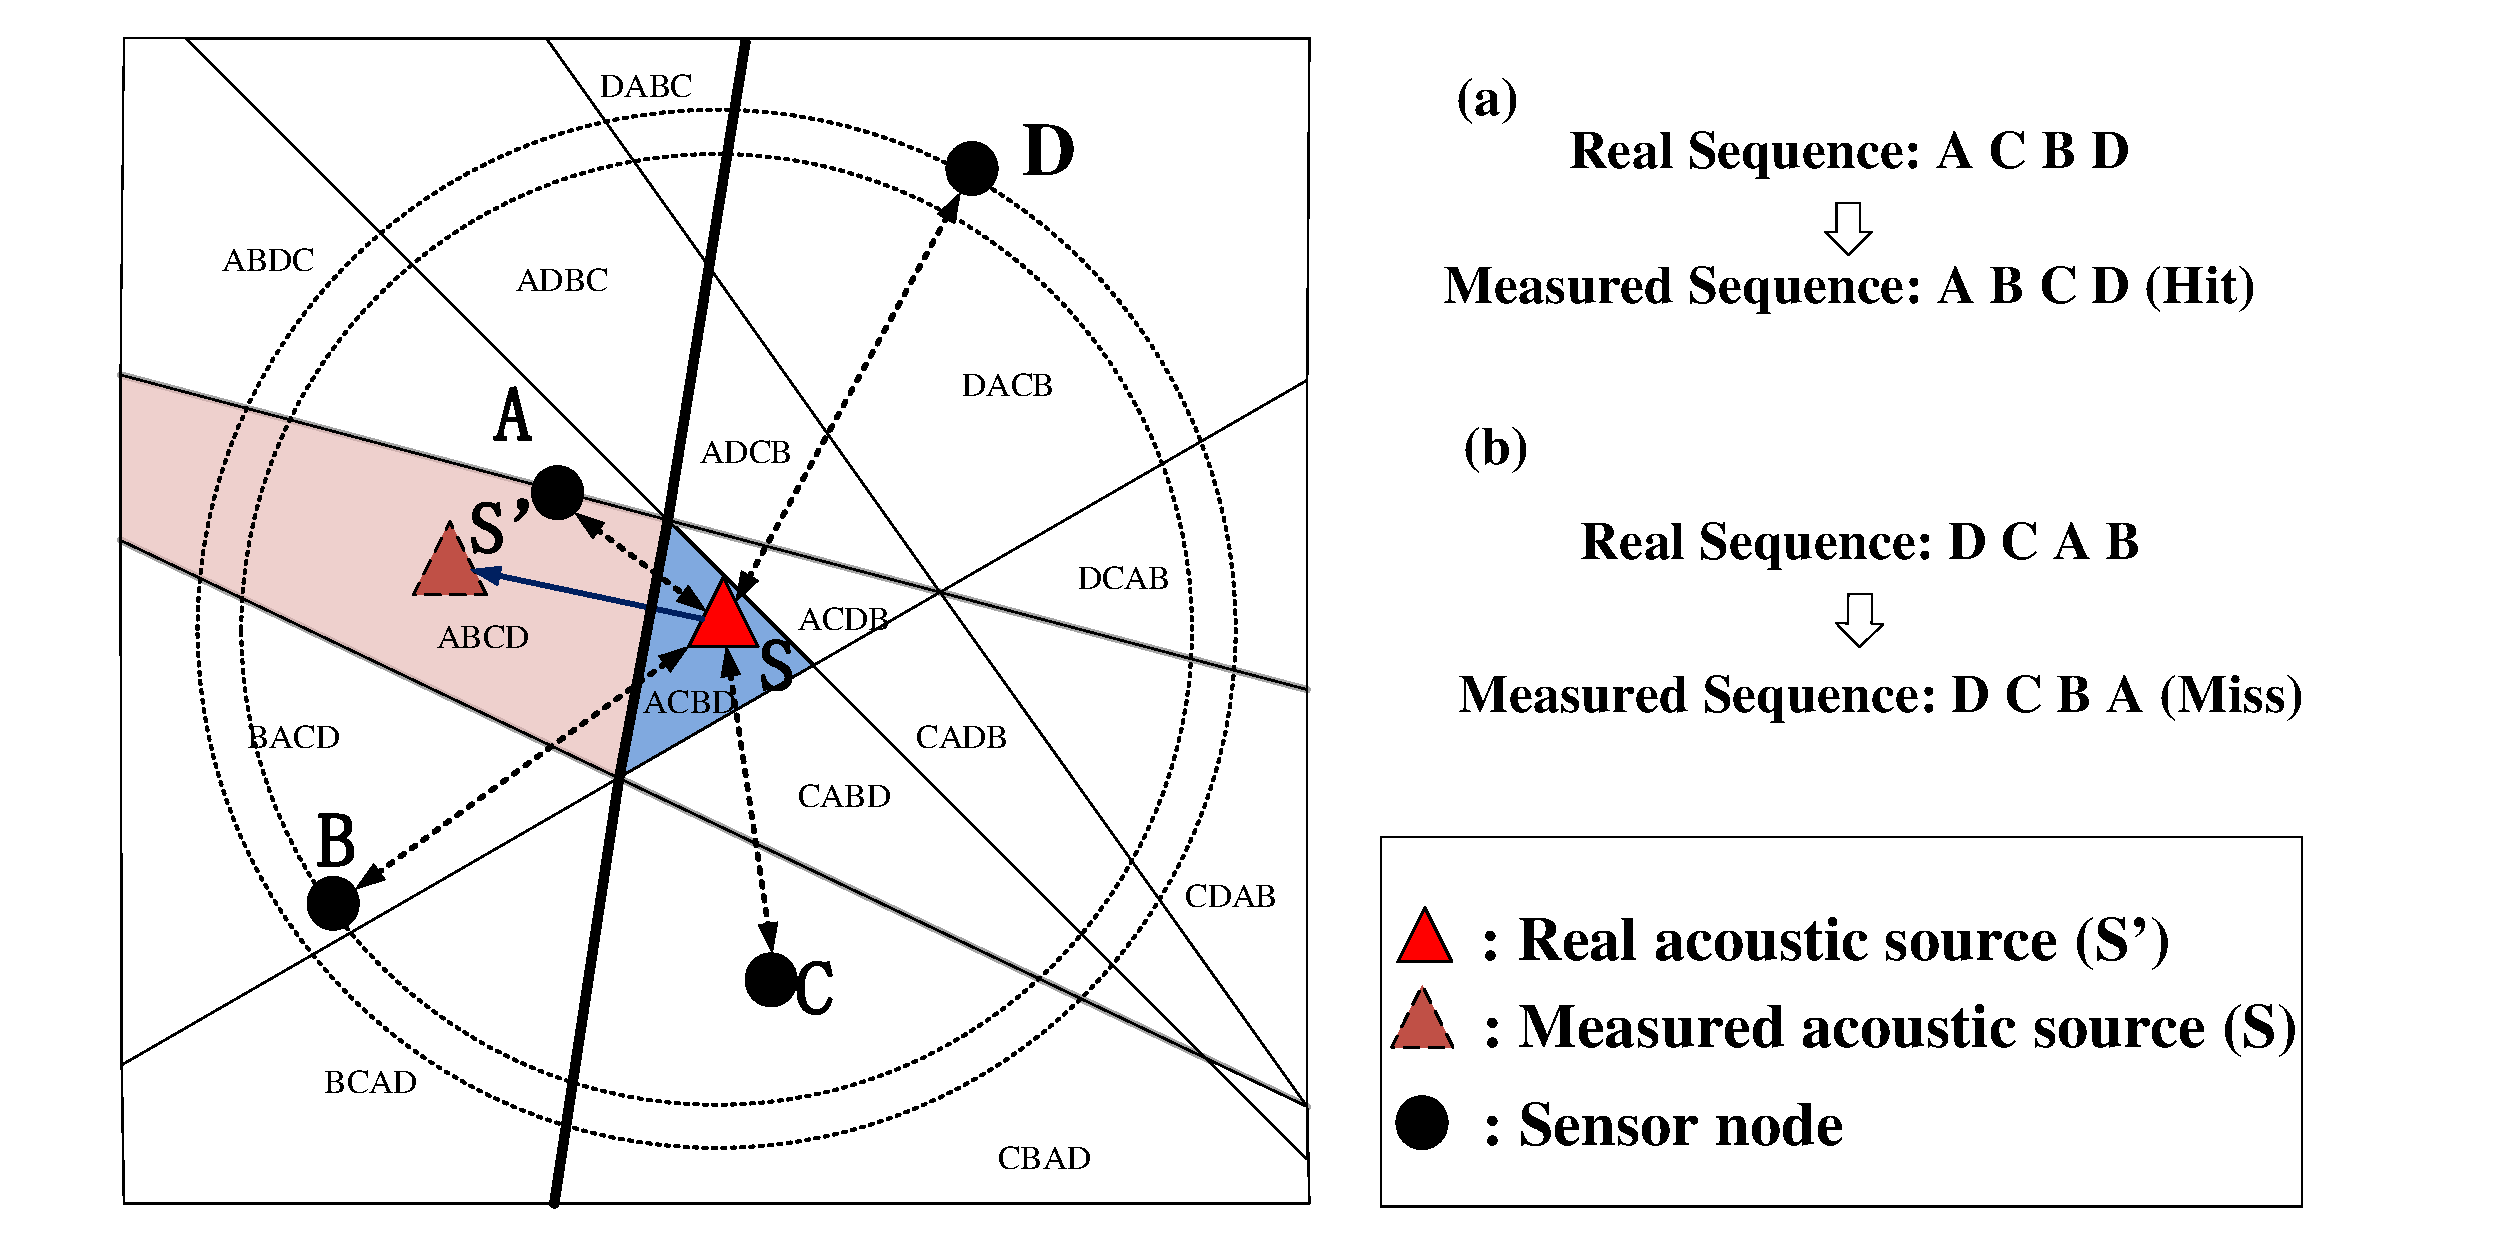
\includegraphics[height=4.5cm]{image/fig2.eps} 
	\vspace{10mm}
    \caption{The basic idea of LPSBL}
	\label{fig2}
    \vspace{-5mm}
    \end{figure}

In practice, solving the inverse problem is extremely difficult. 
In prior research, SBL estimated the location of nodes roughly by using a searching method with heavy computation. 
While in this paper, we carefully formulate Problem 2 as a convex optimization issue and propose an efficient solution which can provide the optimal localization results without significant overhead. 
To the best of our knowledge, this is the first work to leverage convex optimization for solving sequence-based localization problems in sensor networks.





